\documentclass[french, 11pt, a4paper]{article}
\usepackage{xunicode}
\usepackage{fontspec}
\usepackage[frenchb]{babel}
\usepackage[T1]{fontenc}
\usepackage{graphicx}

\author{Julien \textsc{Durillon} \and Alexandre \textsc{Garnier}}
\title{Spécification d'un gestionnaire de services}

\begin{document}

\maketitle

\section{Introduction}

Dans le cadre du module de \emph{Construction formelle du logiciel en B} du
Master ALMA de l'Université de Nantes, nous avons eu à concevoir la
spécification formelle en B d'un système des gestion de services au sein d'un
OS.\\

Il s'agit plus précisément d'une architecture basée sur un ensemble de services
accessibles par un nombre variable de processus, selon que ces services soient
en accès exclusif ou inclusif.
L'accès aux services exclusifs devra être basé sur des profils de processus, de
sorte que seuls les processus dont le profil est reconnu par un service pourront
utiliser celui-ci.

Ce faisant, on distingue trois concepts principaux au sein du projet, à savoir
les services, les processus et les profils.
Dès lors, dans notre travail de conception puis de spécification, nous avons eu
pour objectif principal de refléter cette telle répartition.\\

Dans la suite, après une analyse plus avancée du sujet, nous présenterons la
spécification formelle des différents aspects attendus du logiciel, ainsi que
les différents raffinements et implantations opérées.

Enfin, nous discuterons de la solution finale, des problèmes encontrés dans sa
conception, et des avantages et inconvénients que nous avons pu mettre à jour
quant à l'utilisation de B, et plus spécifiquement d'AtelierB.

\section{Analyse}

\subsection{Les éléments du système}

Pour pouvoir répondre aux conditions du système, nous devons manipuler les
concepts suivants:

\begin{itemize}
  \item processus: un processus identifié par un numéro;
  \item service: un service est utilisé par un processus;
  \item profile: un processus possède un profil; un service peut filtrer les
    processus autorisés via leur profil.
\end{itemize}

\subsection{Première itération sur l'architecture}

Dans la première version, nous avons commencé par créer une machine pour gérer
les processus, leurs profils et les services.
Nous nous sommes rendus compte que cette version était lourde et peu adaptée.

\subsection{Deuxième version : modularisation}

Les concepts \emph{processus} et \emph{profile} sont intimement liés.
Nous allons donc séparer la conception en deux parties: d'un côté la gestion des
processus et de leur profil, de l'autre la gestion des services.

\subsubsection{ProcManager}

La machine ProcManager définit le concept de \emph{processus} et celui de
\emph{profile}.

\subsection{Machine composite}

Pour gérer les différents éléments, une machine Système doit être faite.
Elle va définir les actions haut-niveau qui utiliseront les processus et les
services.

\section{Spécification}

\subsection{Ensembles et relations: diagrammes d'Euler-Venn}

\subsubsection{Gestionnaire de processus}

\begin{figure}[htb]
  \centering
  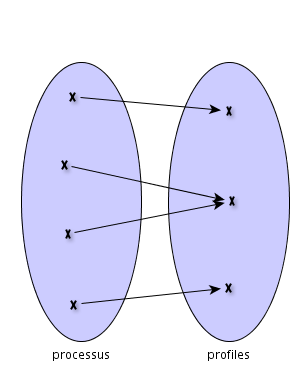
\includegraphics[width=0.4\textwidth]{proc_profile.png}
  \caption{proc_profile: processus --> profiles}
  \label{fig:proc_profile}
\end{figure}

\subsubsection{Gestionnaire de services}

\section{Organisation du travail}
Plusieurs aspects nous ont poussés à travailler ensemble sur le projet: la
gestion des projets dans AtelierB ne nous permettait pas un partage simple des
fichiers de projets; la méthode B nous étant encore assez étrangère, nous avons
préféré travailler ensemble sur les spécifications et sur le développement pour
assurer une meilleure qualité.

Dans la partie processus, il doit être possible de créer et de supprimer un
processus, d'y associer un profil.

Dans la partie service, il doit être possible de déclarer un service, de
l'activer, d'y associer les profils autorisés, d'inscrire des processus à un
service.

\end{document}

